\section{实验结果及分析}
\subsection{仿真图}

\begin{figure}[htbp]
    \centering
    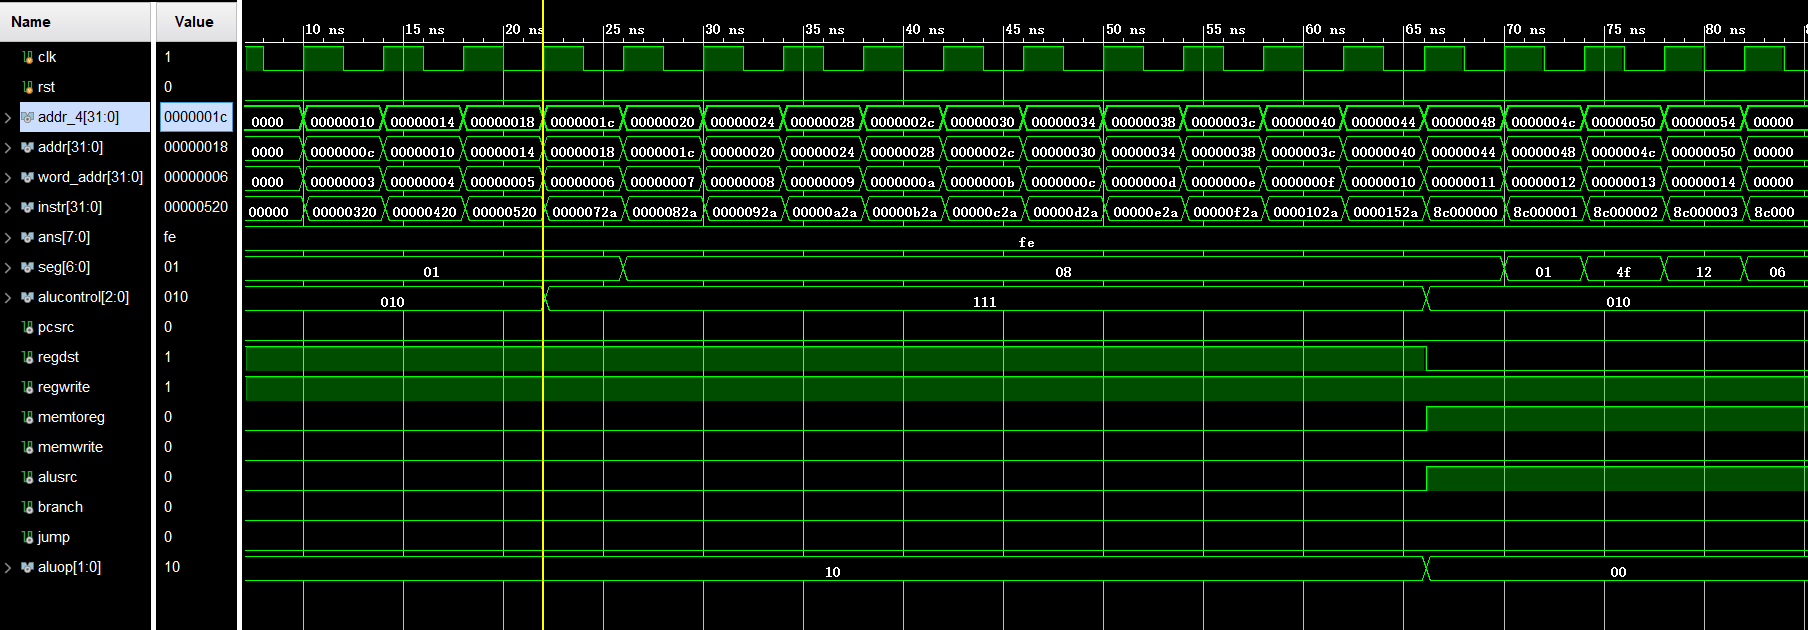
\includegraphics[width=0.8\textwidth]{1.png}
    \caption{仿真图1}
\end{figure}

\begin{figure}[htbp]
    \centering
    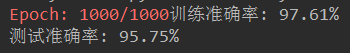
\includegraphics[width=0.8\textwidth]{2.png}
    \caption{仿真图2}
\end{figure}

\textbf{结果分析: }
\begin{enumerate}
    \item PC每个周期自增4,按照顺序得到连续指令。译码后得到正确的控制信号
    \item 上述仿真图中按照R型,lw,sw,beq,addi,jump的顺序进行仿真
    \item 指令为00000520时为add,regdst和regwrite为1,alucontrol为010
    \item 指令为0000072a时为slt,regdst和regwrite为1,alucontrol为111
    \item 指令为8c000001时为lw ,regwrite、memtoreg和alusrc为1,alucontrol为010
    \item 指令为ac000001时为sw ,memwrite和alusrc为1,alucontrol为010
    \item 指令为10000001时为beq,branch为1,alucontrol为110
    \item 指令为20000001时为addi,regwrite和alusrc为1,alucontrol为010
    \item 指令为08000001时为jump,jump为1
\end{enumerate}

\subsection{上板图}

\textbf{结果分析: }
\begin{enumerate}
    \item 每一秒切换一条指令,按照coe中的顺序显示在七段数码管上,并显示11位的控制信号
    \item led[10:8]:alucontrol
    \item led[7:0]:{branch,jump,regwrite,regdst,alusrc,pcsrc,memwrite,memtoreg}
    \item 如图所示,信号显示正确
\end{enumerate}

\begin{figure}[htbp]
    \centering
    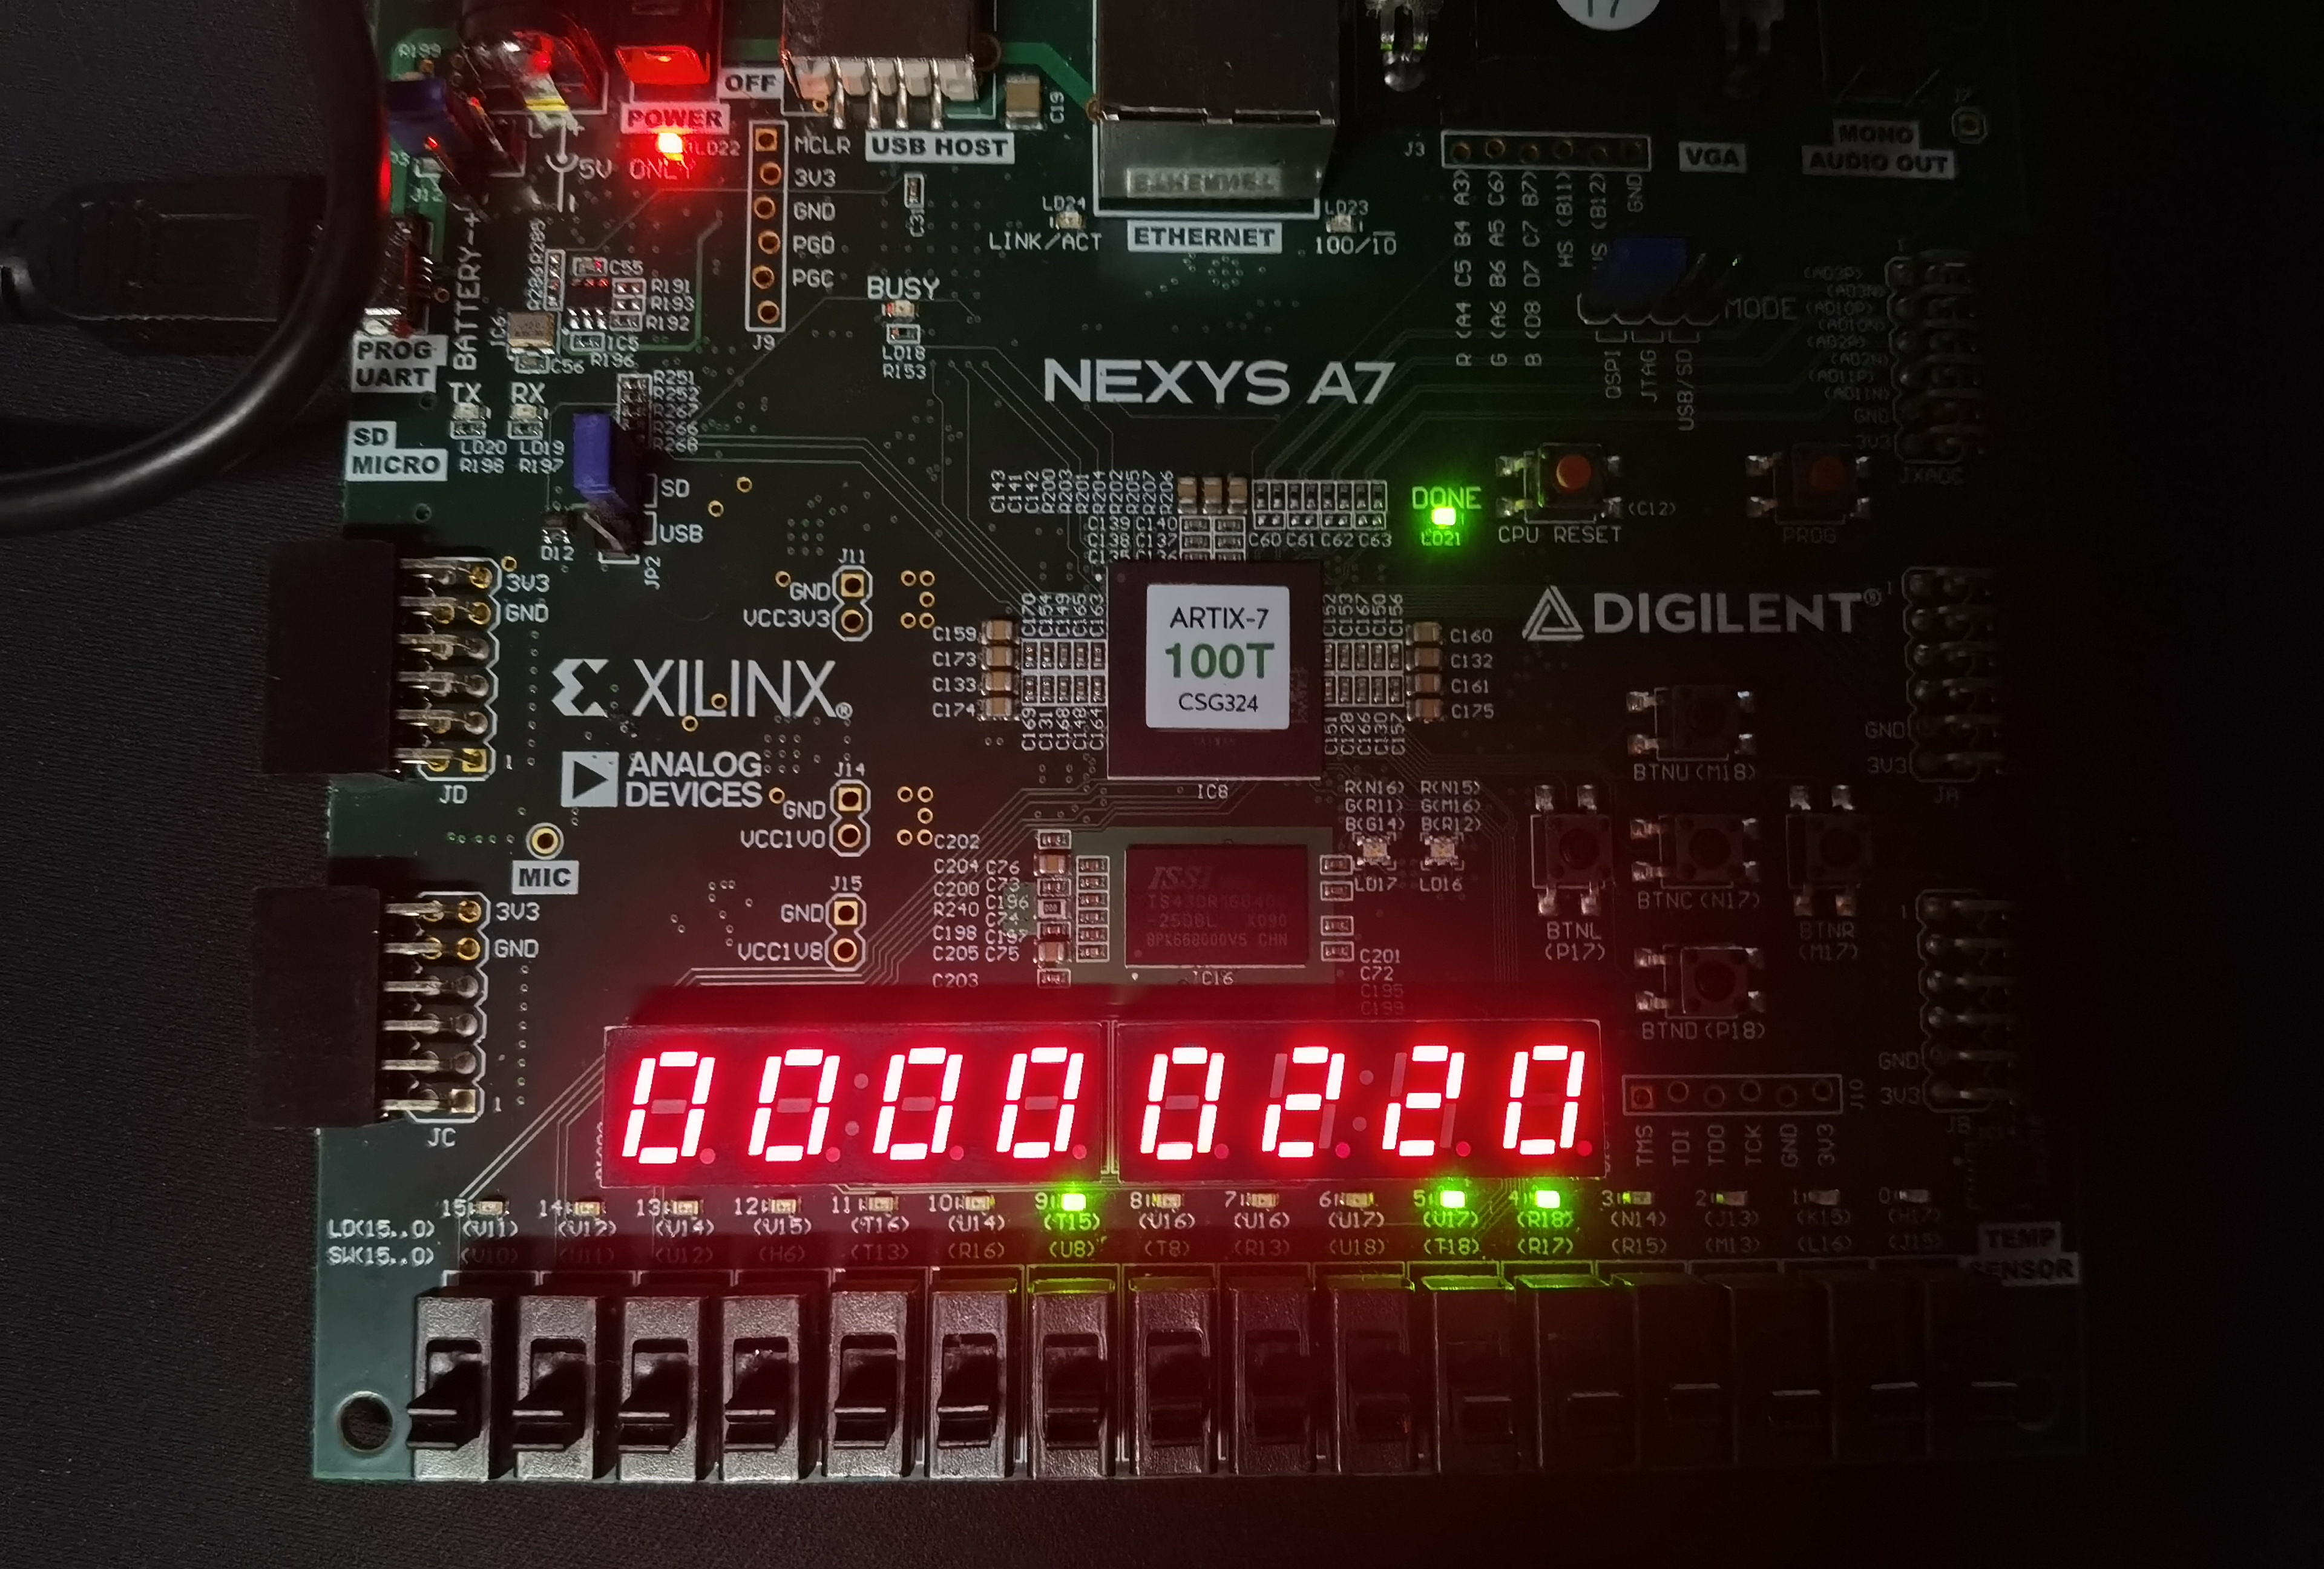
\includegraphics[width=0.8\textwidth]{0020_add.jpg}
    \caption{add}
\end{figure}

\begin{figure}[htbp]
    \centering
    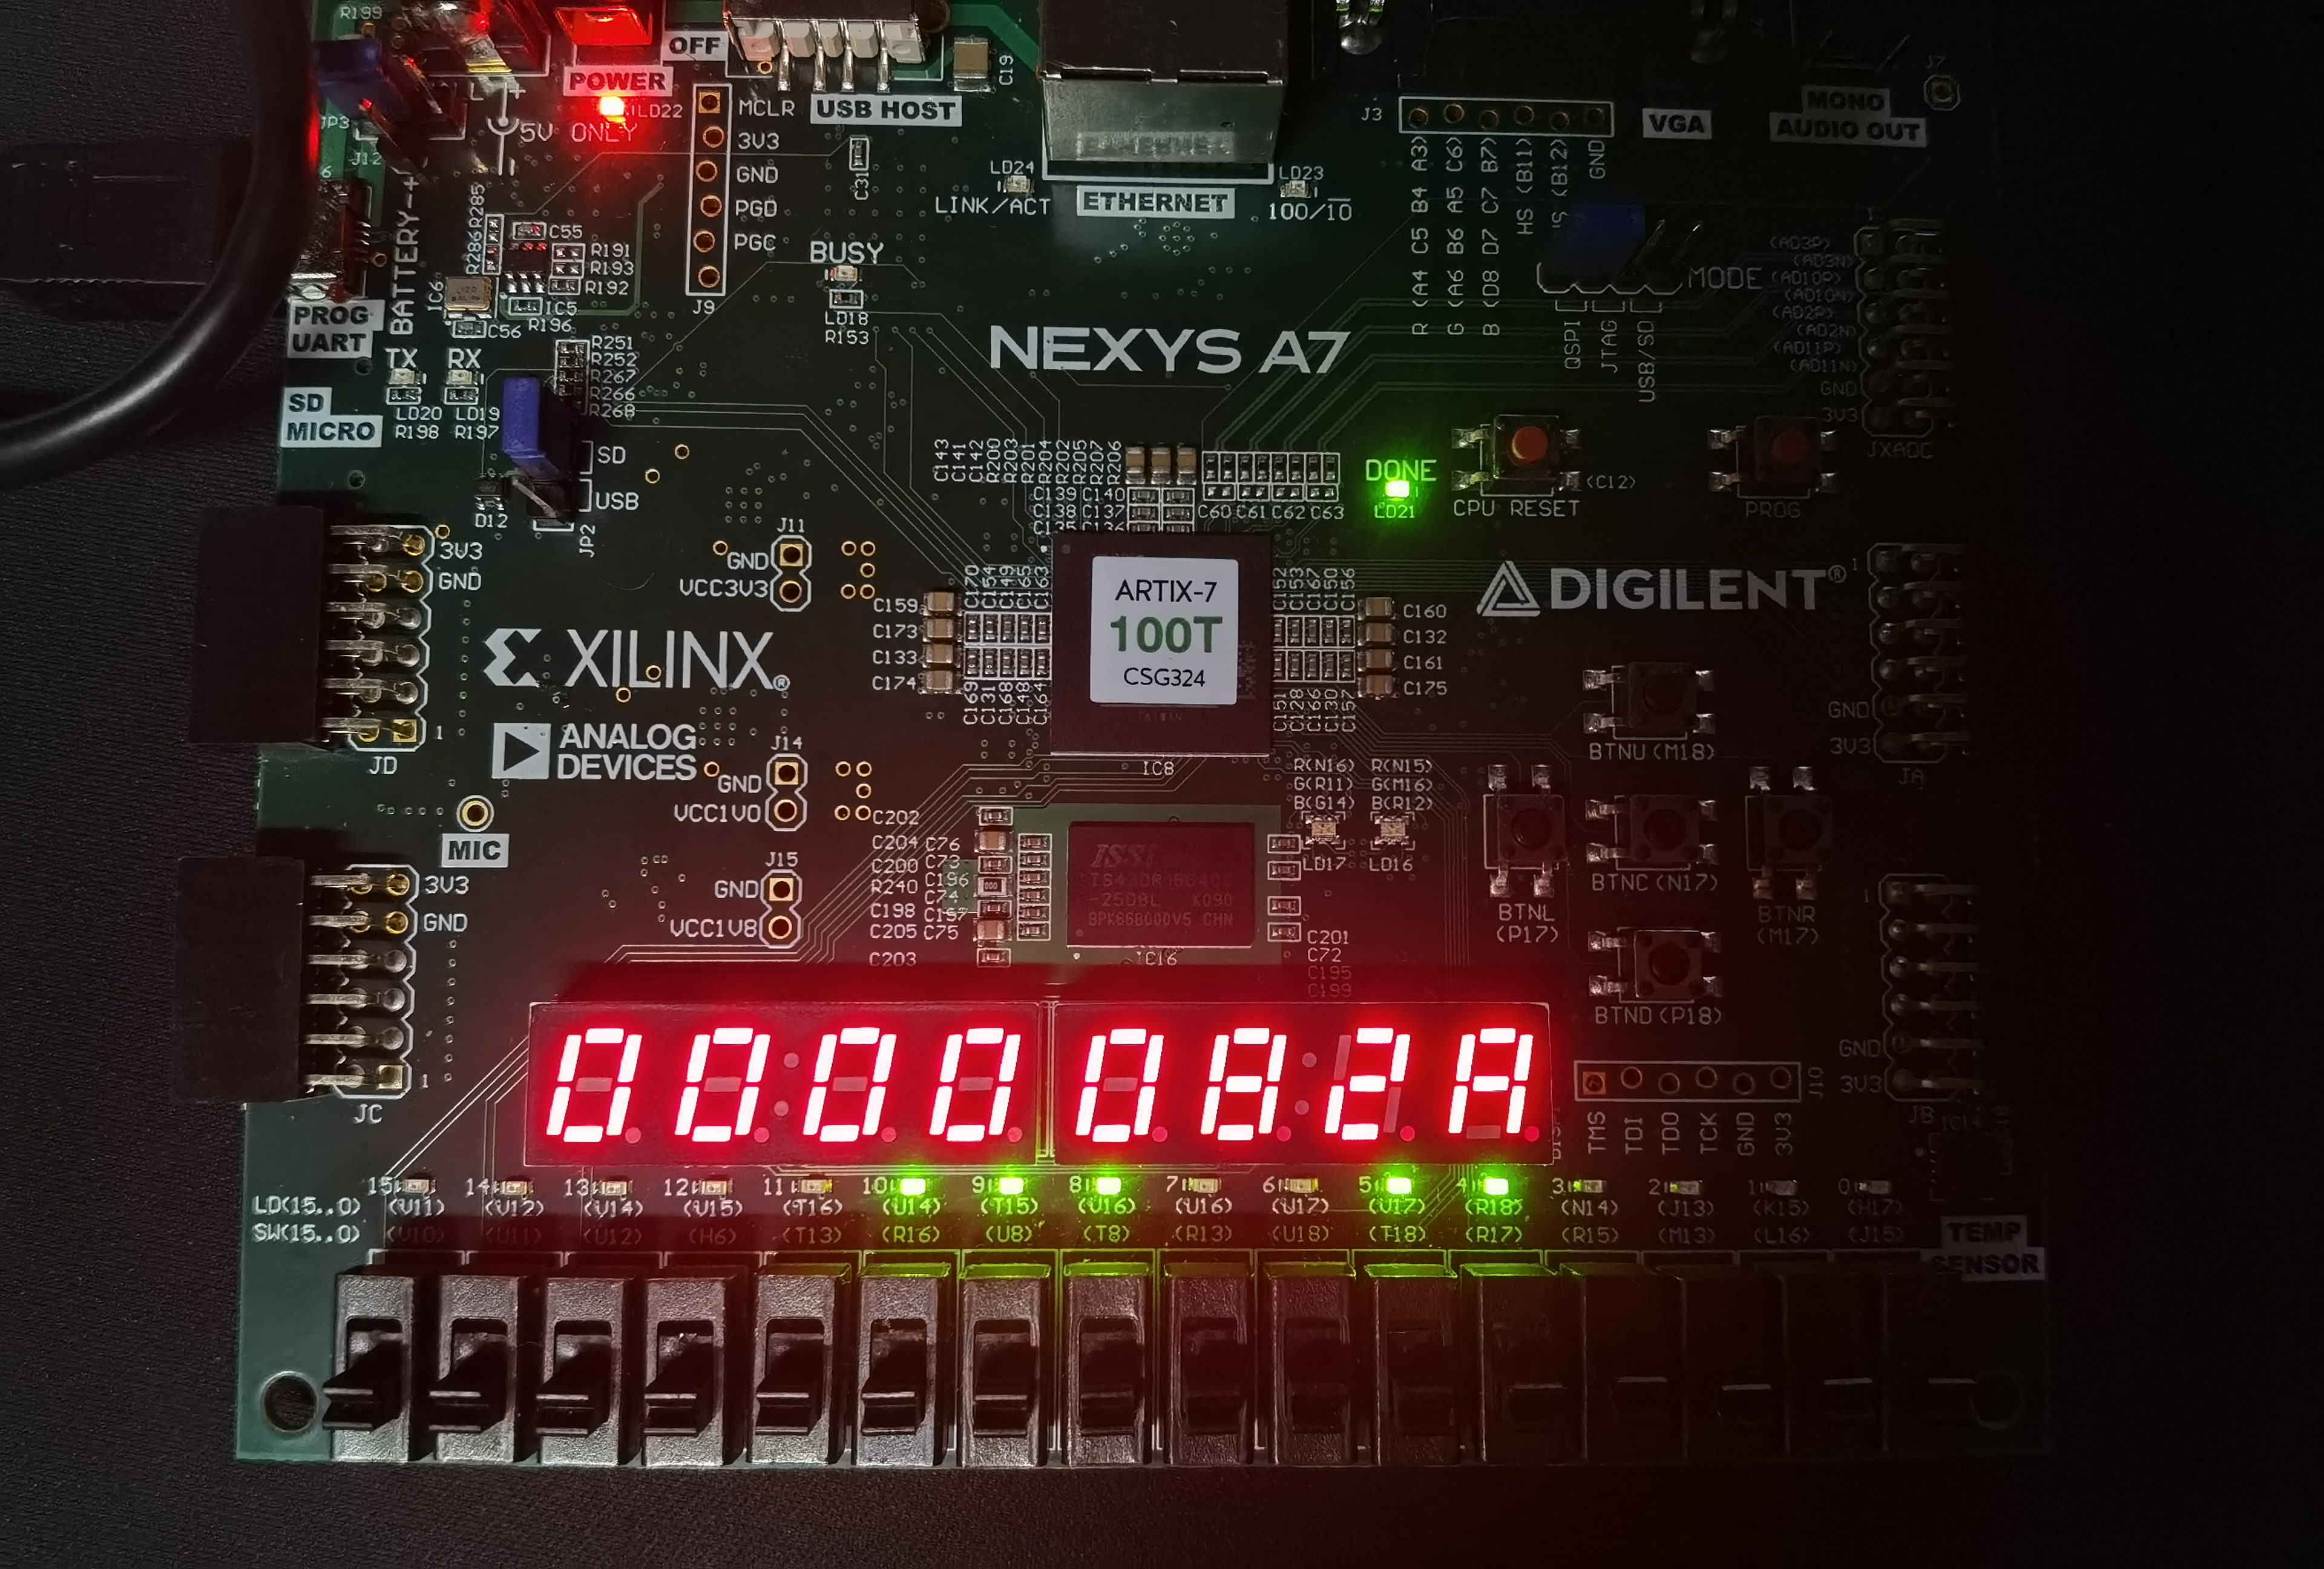
\includegraphics[width=0.8\textwidth]{002a_slt.jpg}
    \caption{slt}
\end{figure}

\begin{figure}[htbp]
    \centering
    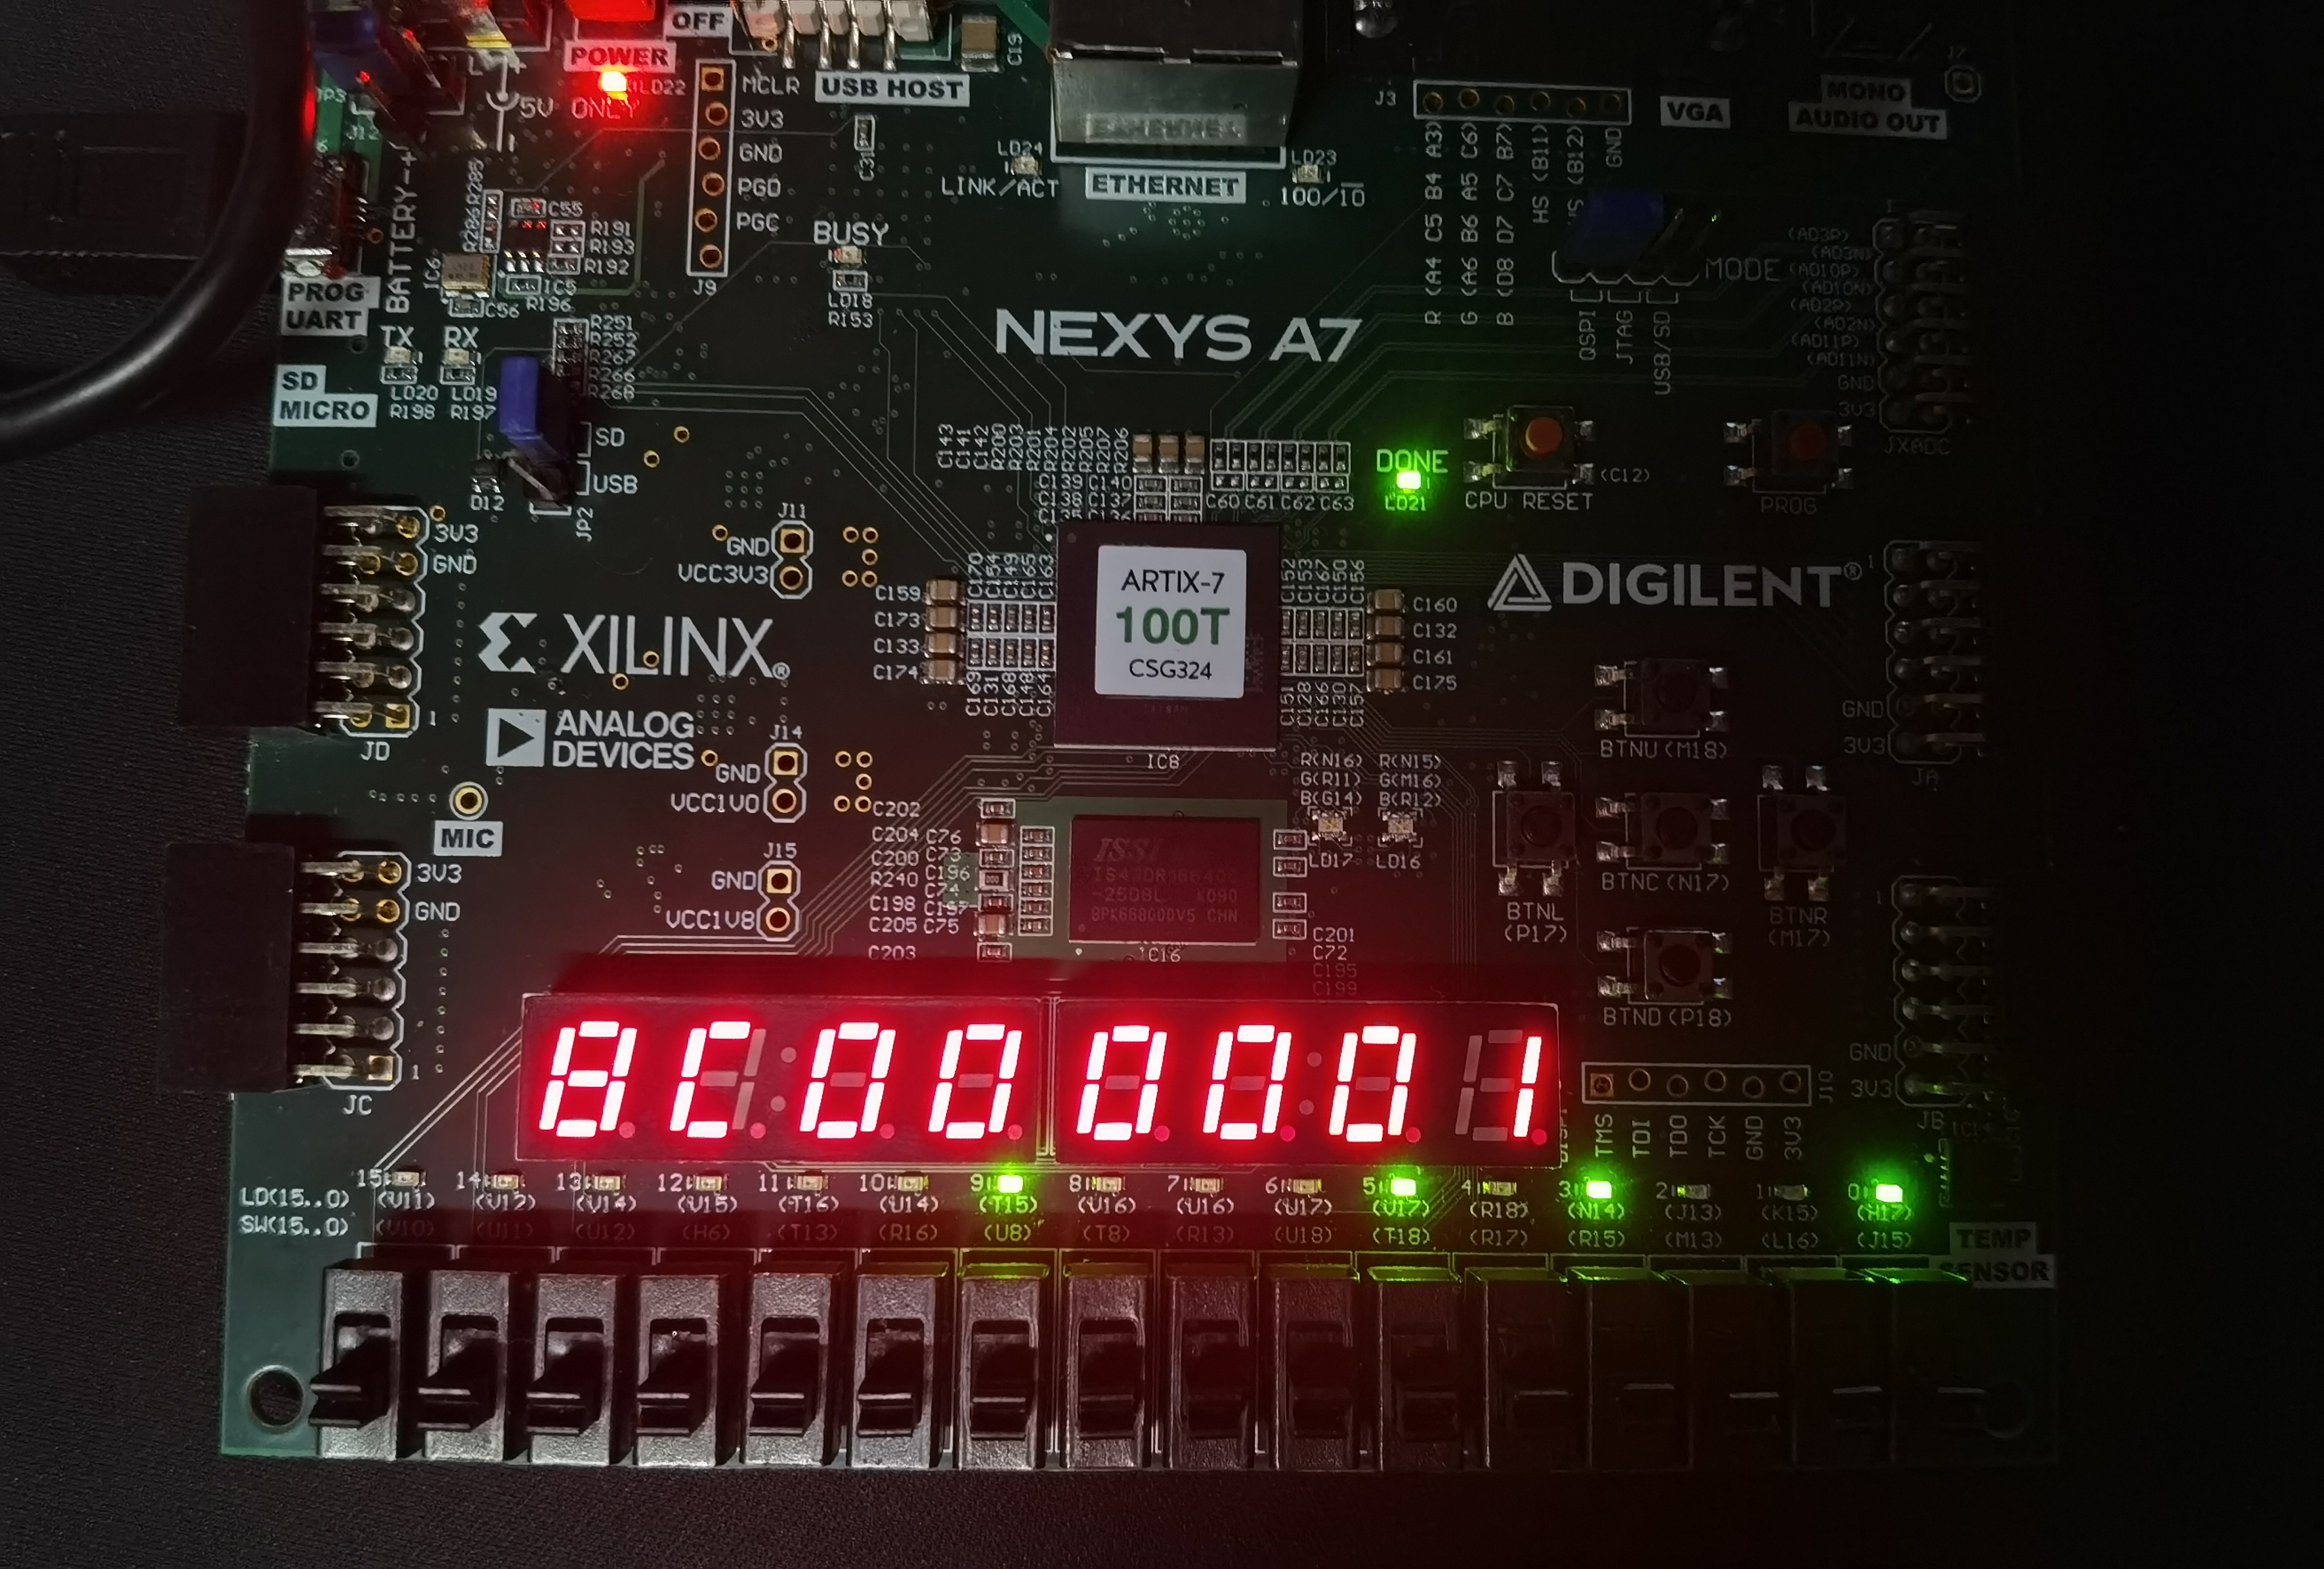
\includegraphics[width=0.8\textwidth]{8c_lw.jpg}
    \caption{lw}
\end{figure}

\begin{figure}[htbp]
    \centering
    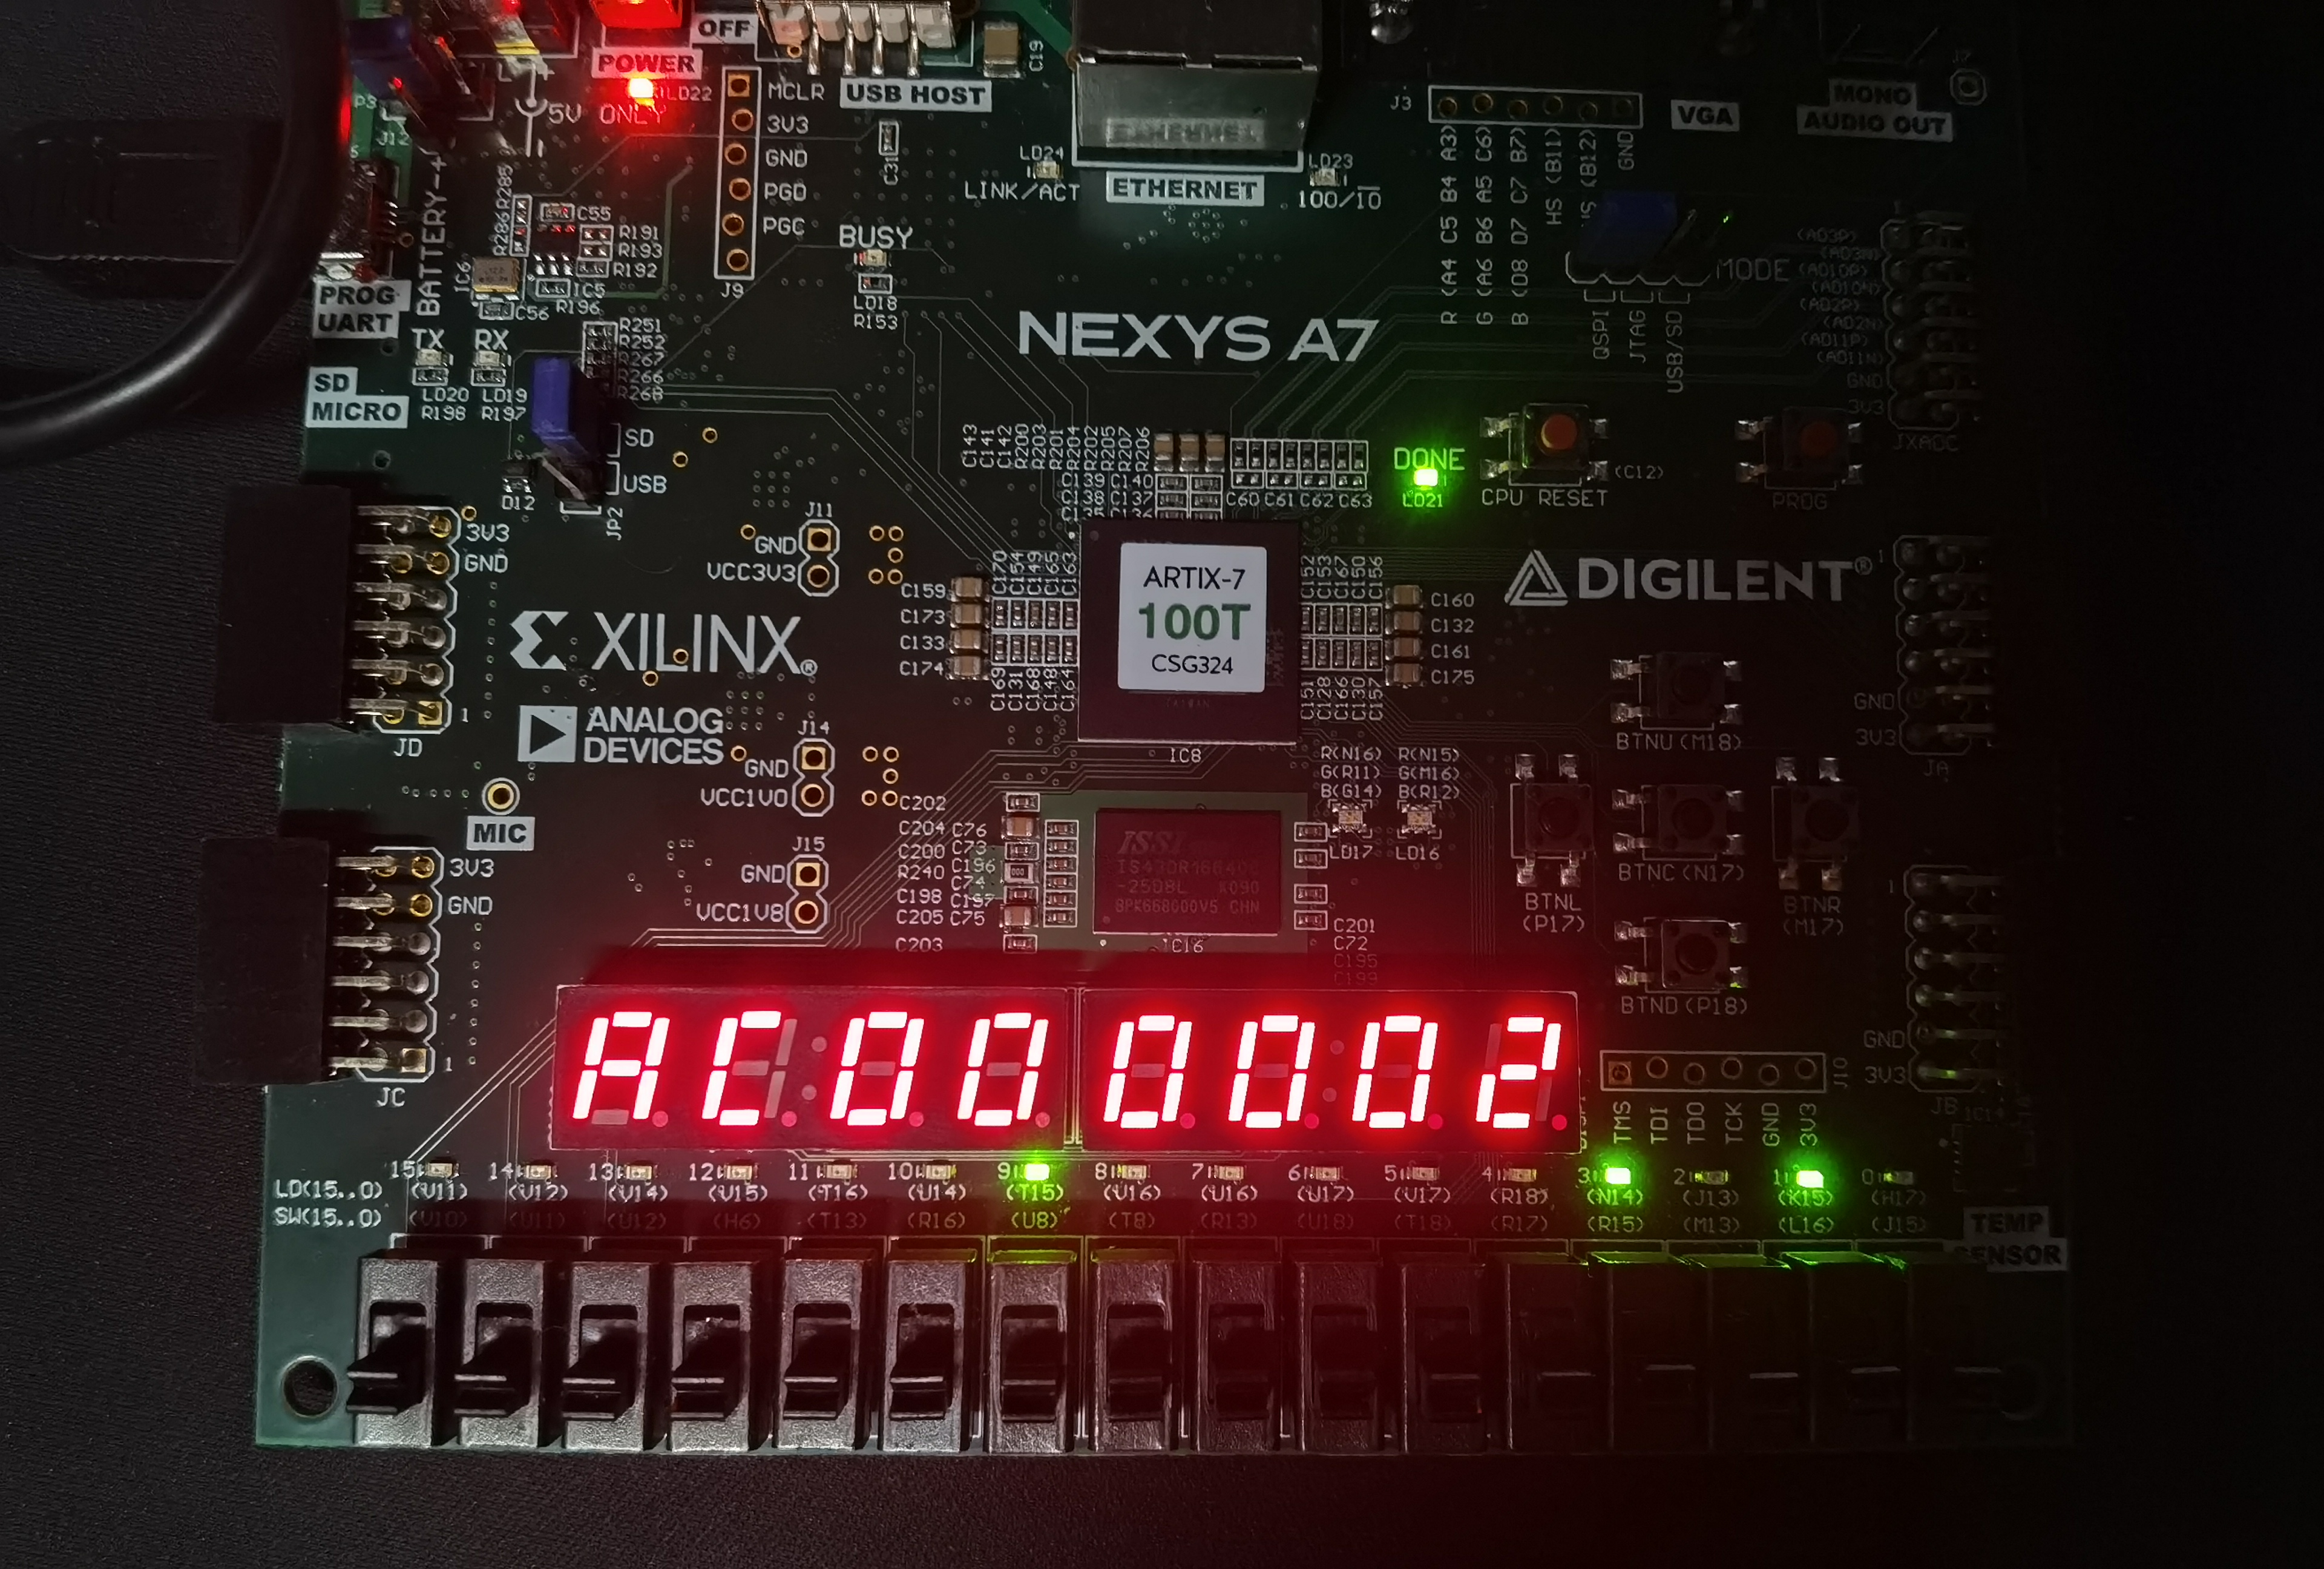
\includegraphics[width=0.8\textwidth]{ac_sw.jpg}
    \caption{sw}
\end{figure}

\begin{figure}[htbp]
    \centering
    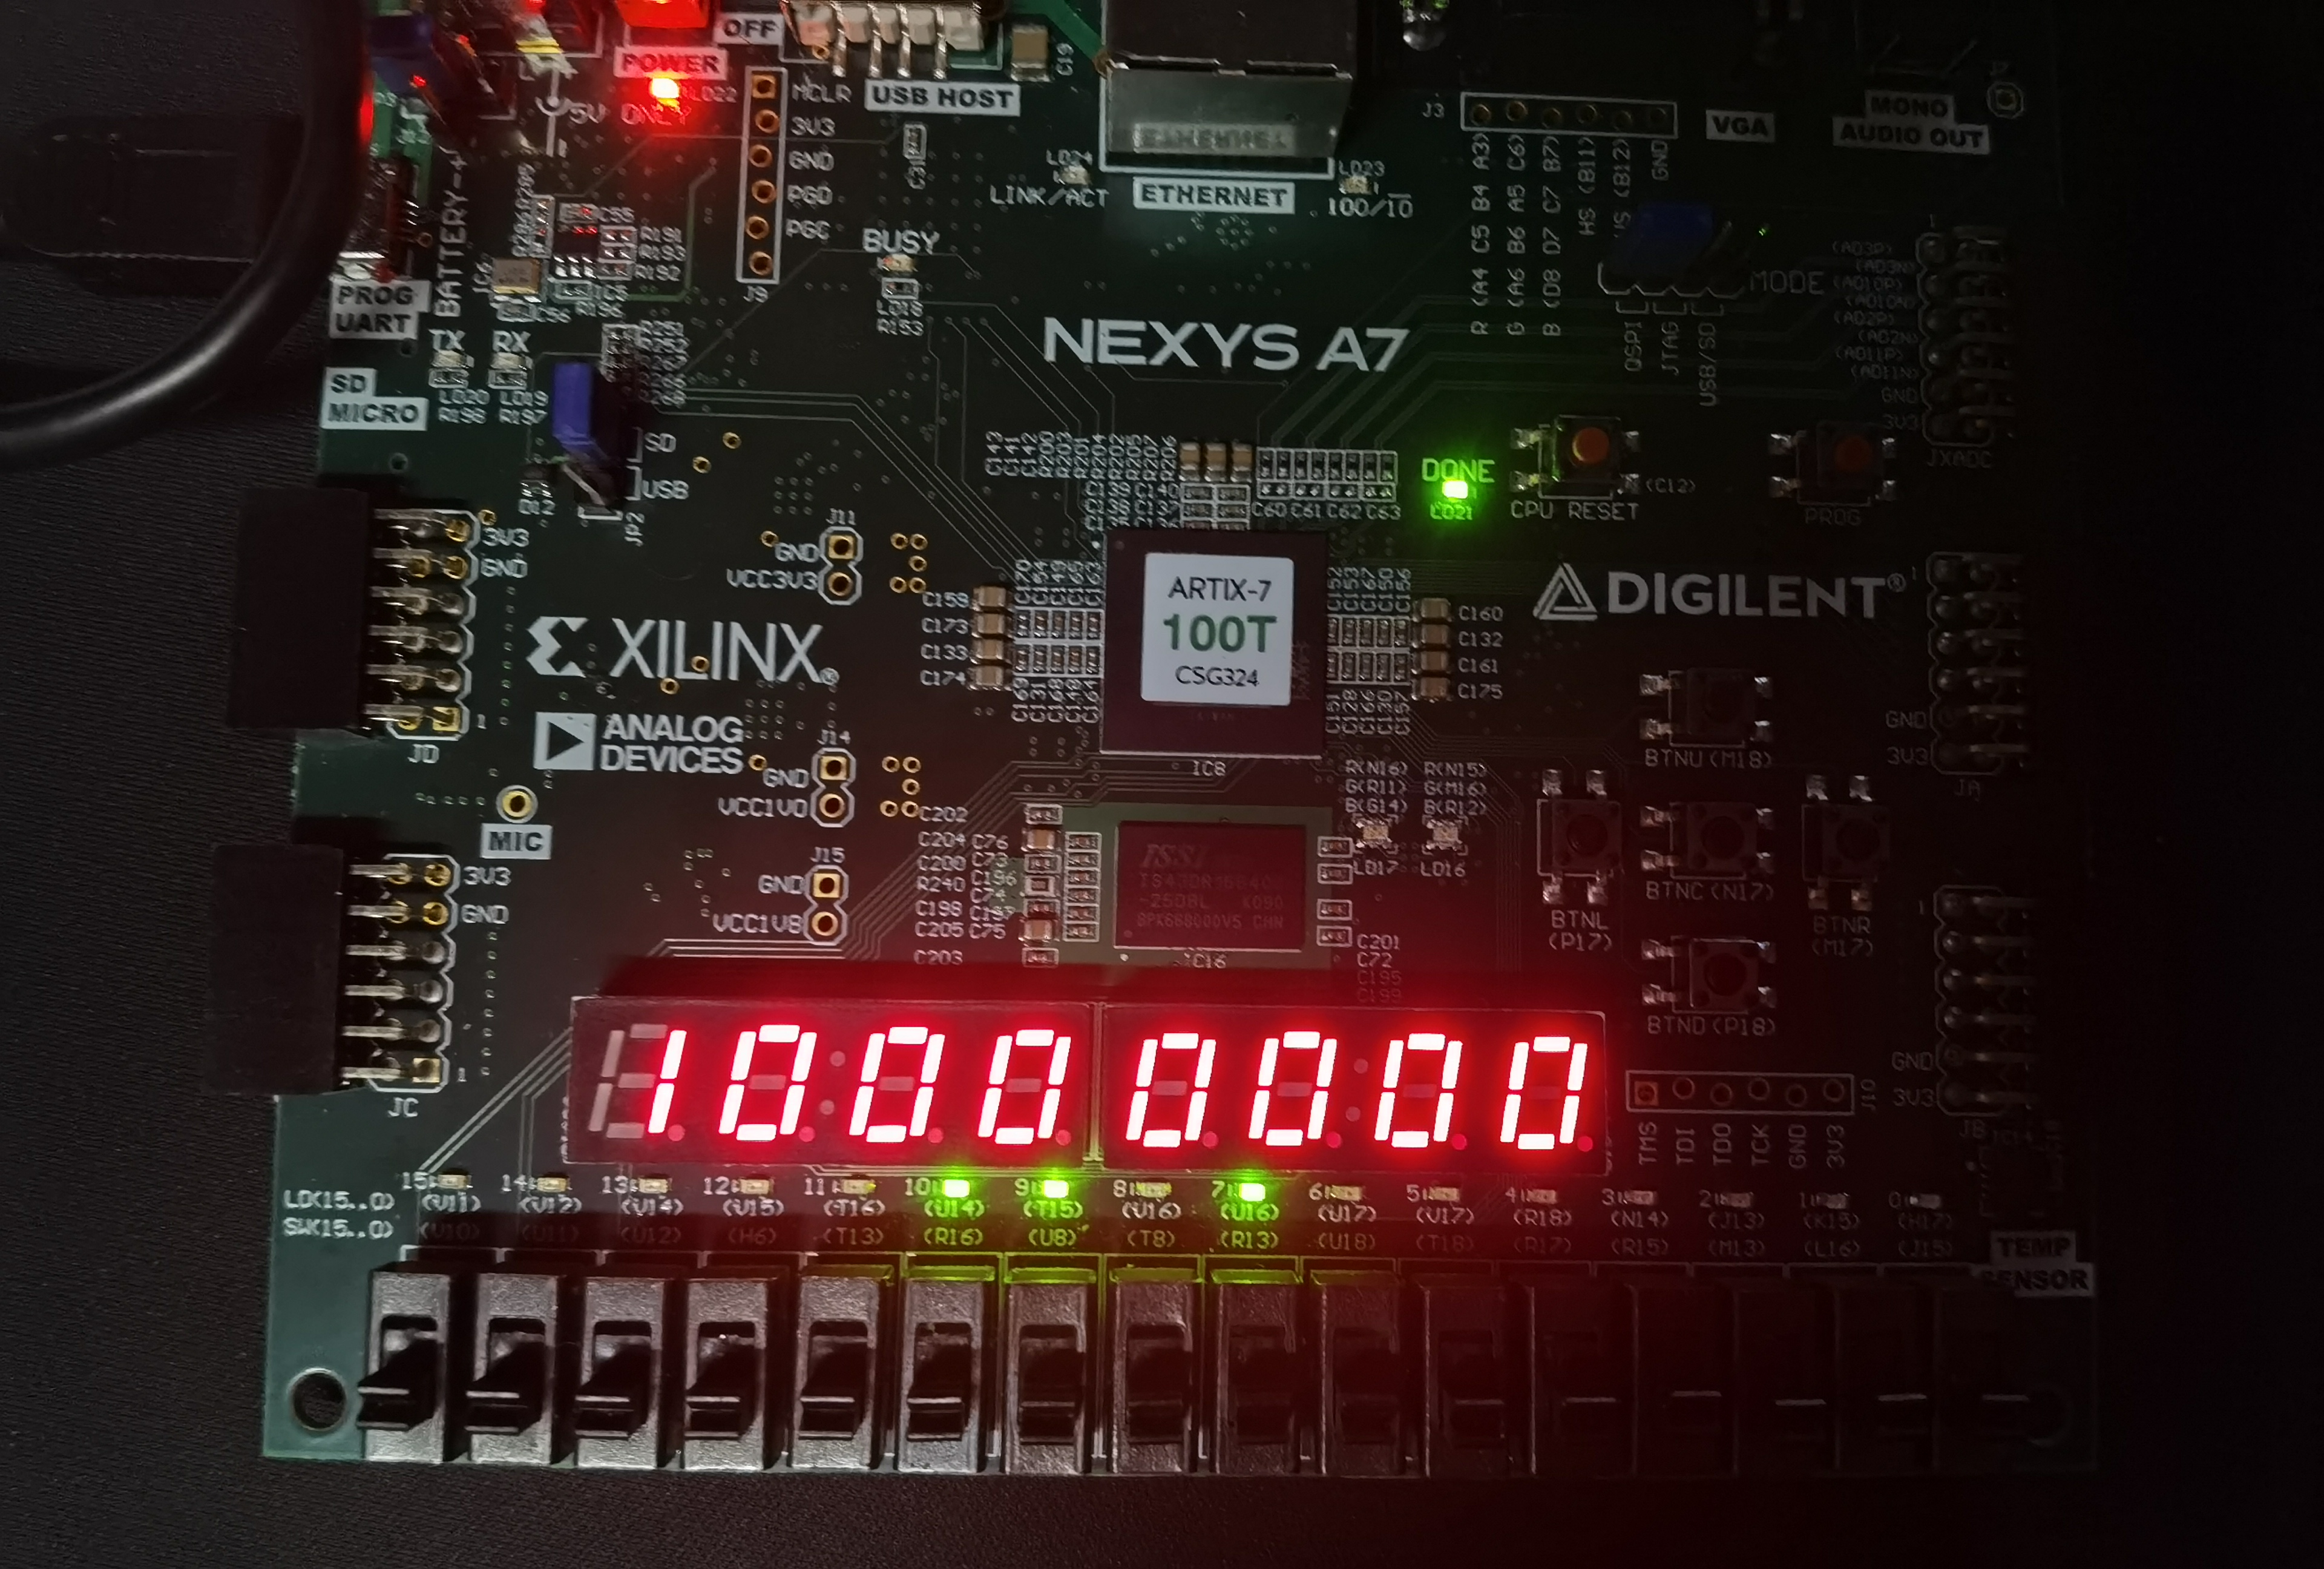
\includegraphics[width=0.8\textwidth]{10_beq.jpg}
    \caption{beq}
\end{figure}

\begin{figure}[htbp]
    \centering
    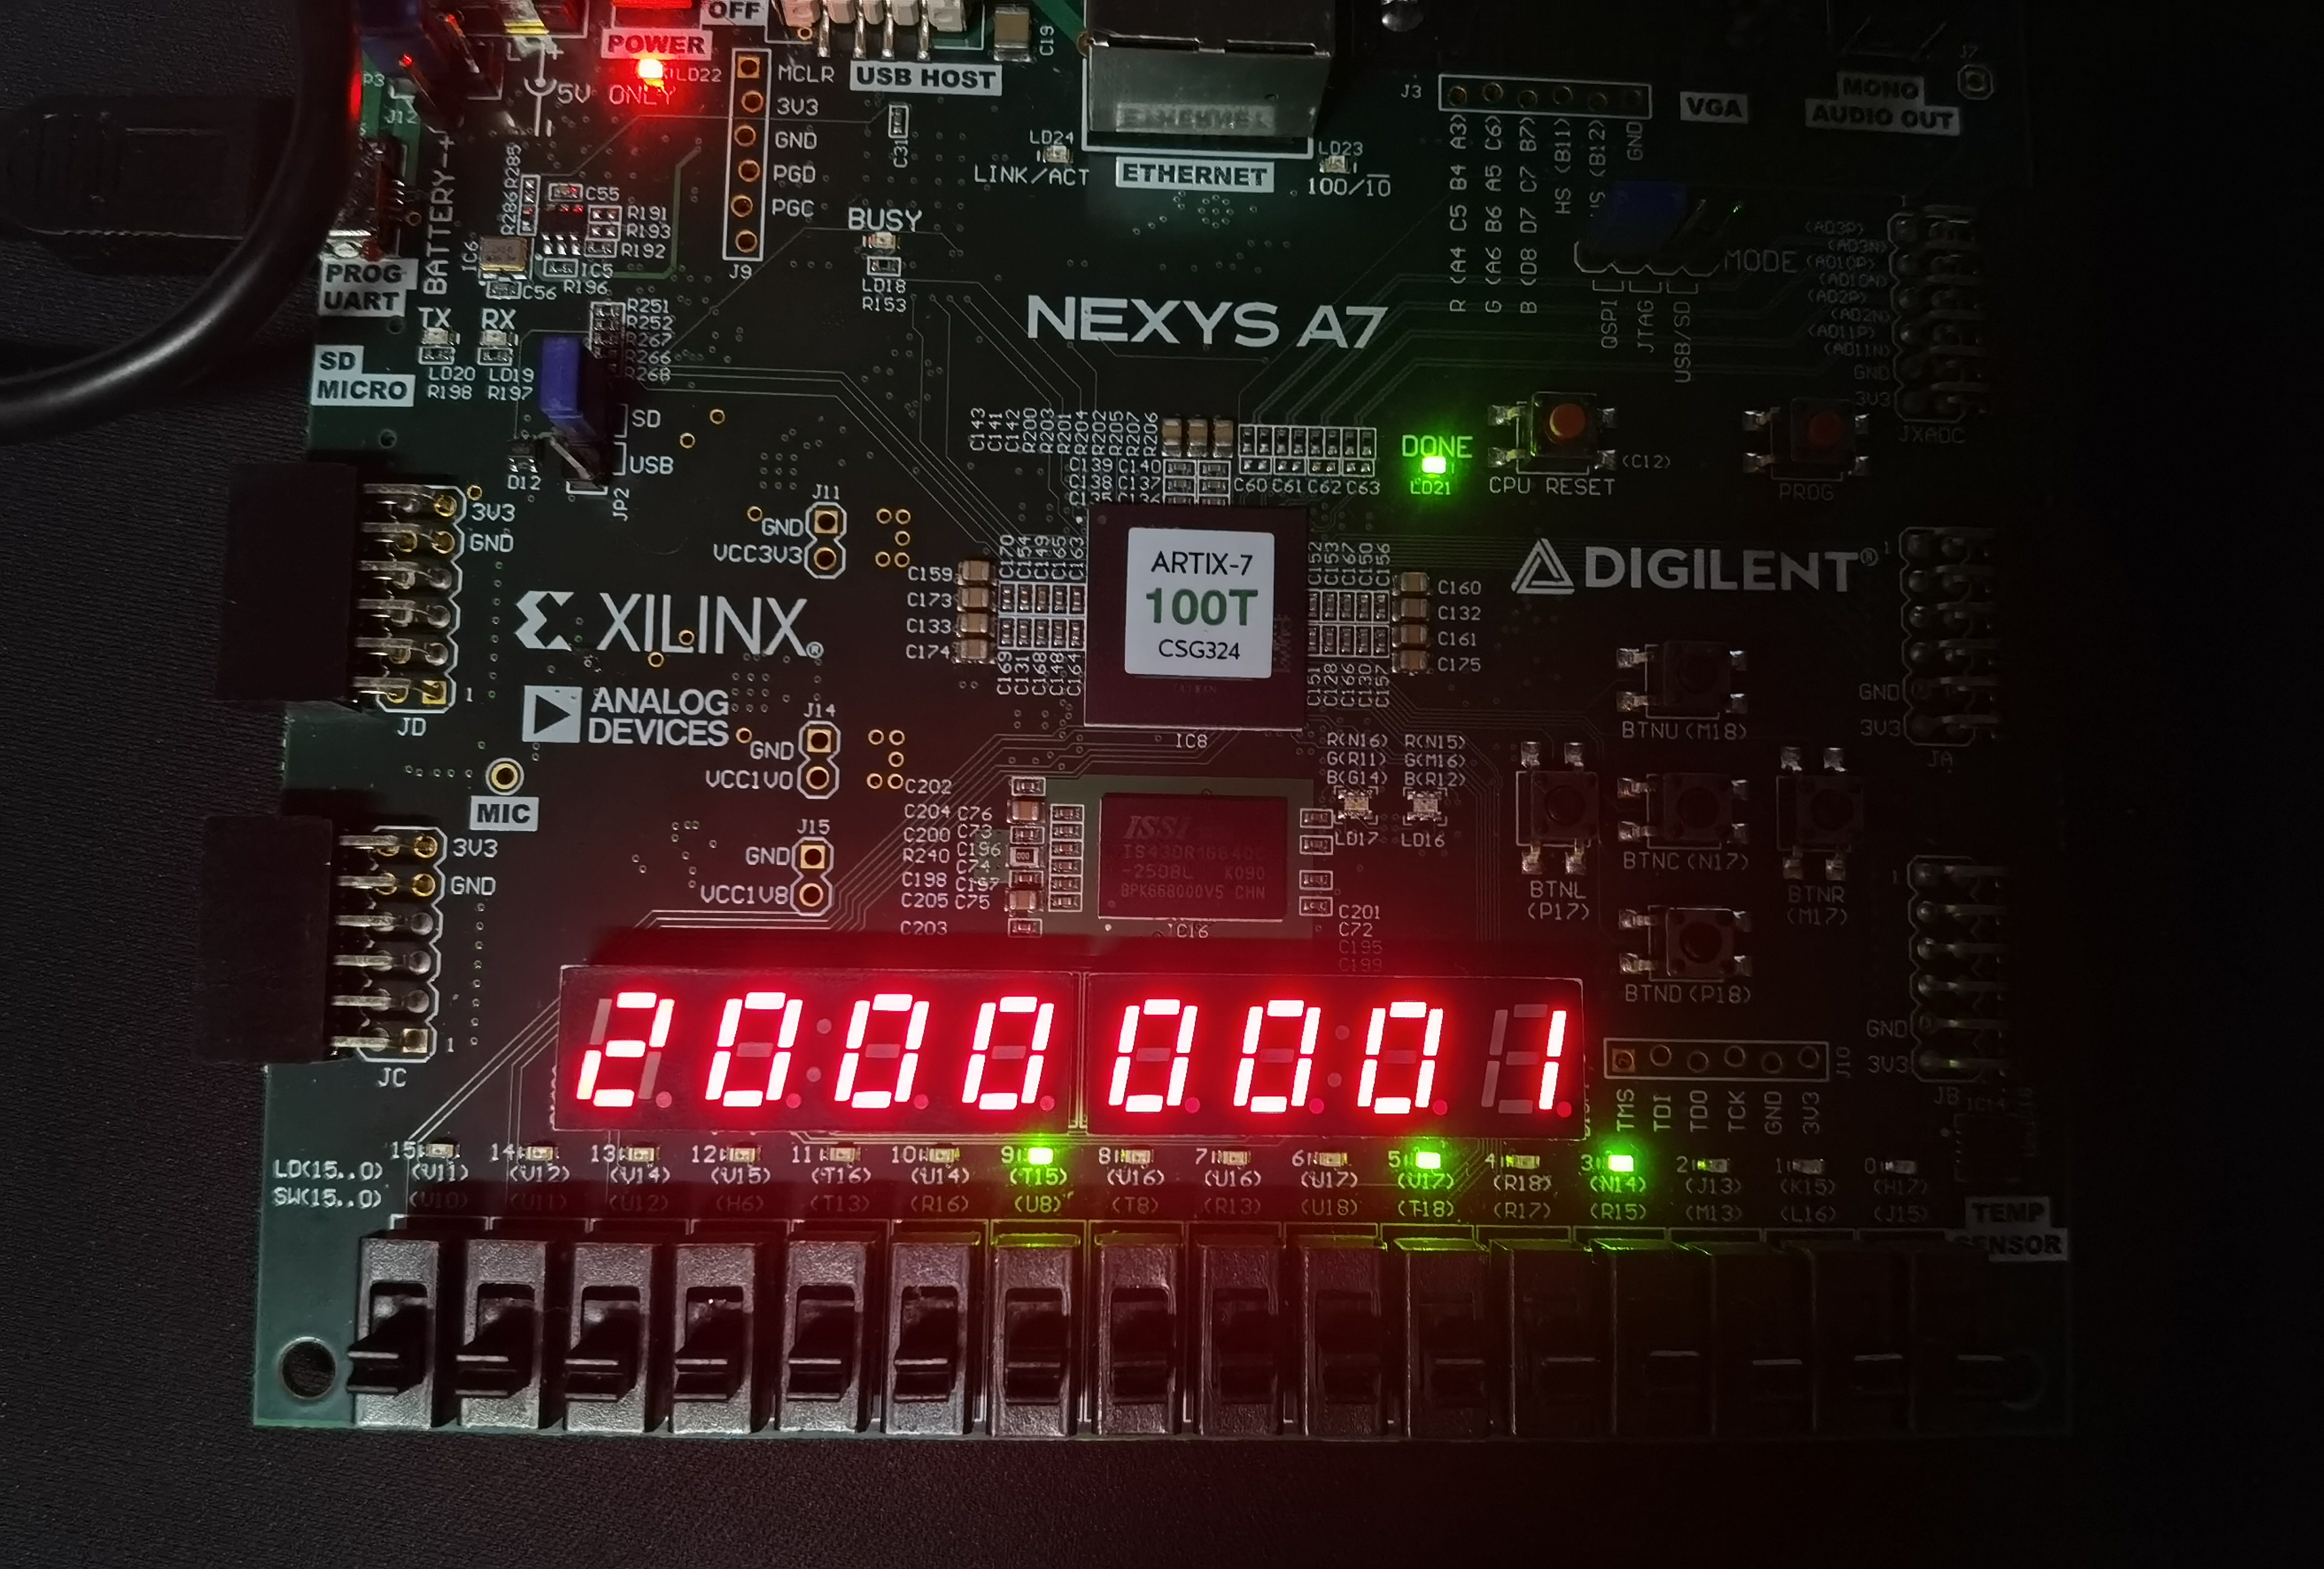
\includegraphics[width=0.8\textwidth]{20_addi.jpg}
    \caption{addi}
\end{figure}

\newpage
\subsection{控制台输出}
